\documentclass[a4paper,12pt]{article}
\usepackage{amsmath,amssymb,amsfonts,amsthm}
\usepackage{tikz}
\usepackage [utf8] {inputenc}
\usepackage [T2A] {fontenc} 
\usepackage[russian]{babel}
\usepackage{cmap}
\usepackage{listings}
\usepackage{color}

\definecolor{mygreen}{rgb}{0,0.6,0}
\definecolor{mygray}{rgb}{0.5,0.5,0.5}
\definecolor{mymauve}{rgb}{0.58,0,0.82} 

\lstdefinestyle{customc}{
	belowcaptionskip=1\baselineskip,
	breaklines=true,
	frame=L,
	xleftmargin=\parindent,
	language=Python,
	showstringspaces=false,
	basicstyle=\footnotesize\ttfamily,
	keywordstyle=\bfseries\color{green!40!black},
	commentstyle=\itshape\color{purple!40!black},
	identifierstyle=\color{blue},
	stringstyle=\color{orange},
}


\newtheorem{defenition}{Определение}
\newtheorem{theorem}{Теорема}
\newtheorem{problem}{Задача}

\lstset{escapechar=@,style=customc}

% Так ссылки в PDF будут активны
\usepackage[unicode]{hyperref}

% вы сможете вставлять картинки командой \includegraphics[width=0.7\textwidth]{ИМЯ ФАЙЛА}
% получается подключать, как минимум, файлы .pdf, .jpg, .png.
\usepackage{graphicx}
% Если вы хотите явно указать поля:
\usepackage[margin=1in]{geometry}
% Или если вы хотите задать поля менее явно (чем больше DIV, тем больше места под текст):
% \usepackage[DIV=10]{typearea}

\usepackage{fancyhdr}

\newcommand{\bbR}{\mathbb R}%теперь вместо длинной команды \mathbb R (множество вещественных чисел) можно писать короткую запись \bbR. Вместо \bbR вы можете вписать любую строчку букв, которая начинается с '\'.
\newcommand{\eps}{\varepsilon}
\newcommand{\bbN}{\mathbb N}
\newcommand{\dif}{\mathrm{d}}

\pagestyle{fancy}
\makeatletter % сделать "@" "буквой", а не "спецсимволом" - можно использовать "служебные" команды, содержащие @ в названии
\fancyhead[L]{\footnotesize Информатика\\ Внимание: конспект не проверялся преподавателями —- всегда используйте рекомендуемую литературу при подготовке к экзамену!}%Это будет написано вверху страницы слева
\fancyhead[R]{}
\fancyfoot[L]{}%имя автора будет написано внизу страницы слева
\fancyfoot[R]{\thepage}%номер страницы —- внизу справа
\fancyfoot[C]{ Замечания и предложения просьба писать на \href{mailto:pulsar@phystech.edu}{pulsar@phystech.edu}}%по центру внизу страницы пусто

\renewcommand{\maketitle}{%
	\noindent{\bfseries\scshape\large\@title\ \mdseries\upshape}\par
	\noindent {\large\itshape\@author}
	\vskip 2ex}
\makeatother
\def\dd#1#2{\frac{\partial#1}{\partial#2}}
\def\ddd#1#2#3{\frac{\partial^2#1}{\partial#2\partial#3}}

\title{Графы. IV} 
\author{Тимофей Хирьянов} 
\date{27 февраля 2016 г.}

\begin{document}
	\maketitle
	\begin{defenition}
		Ориентированный граф --- граф, у ребер которого есть начало и конец.
	\end{defenition}
	\begin{defenition}
		Сильно связный граф --- граф, в котором существует (ориентированный) путь из любой вершины в любую другую.
	\end{defenition}
	\section{Топологическая сортировка}
		\subsection{Алгоритм Кана}
			Пусть дан бесконтурный ориентированный простой граф. Через $A(v)$ обозначим множество вершин такихб из которых есть дуга в вершину $v$.
			Пусть P --- искомая последовательность вершин.
			\newline
			
			пока $|P| < |V|$:\newline 
				выбрать любую $v$ такую, что $A(v) = $ и $v \notin P$\newline 
				$P \Leftarrow P, v$\newline 
				удалить $v$ из всех $A(u), u \neq v$
			\newline
			
			
			Наличие хотя бы одного контура в графе приведёт к тому, что на определённой итерации цикла не удастся выбрать новую вершину v.
	\begin{defenition}
		Корневое дерево --- дерево с отмеченной вершиной.
	\end{defenition}
	\begin{defenition}
		Высота корневого дерева --- максимальное количество ребер в простом пути от корня к вершинам.
	\end{defenition}
	\begin{defenition}
		Двоичное дерево --- дерево, у каждой вершины не более чем два потомка.
	\end{defenition}
	
	Реализуем класс дерева. Для этого сделаем вспомогательный класс вершины с полями левой, правой и родительских вершин. В классе дерева реализуем метод распечатки дерева, поиска вершины по ключу,  добавления и удаления вершины. Также будет полезным метод добавления пары вершин и ребра между ними.
	\lstinputlisting[language=Python]{binarytree.py}
	
	\begin{defenition}
		Несбалансированное дерево --- дерево с различной длинной поддеревьев.
	\end{defenition}
	Что делать в случае несбалансированного дерева? Нужно совершить правый поворот.
	\begin{defenition}
		Правый поворот --- изменение вершины дерева с сохранением упорядоченности.
	\end{defenition}
	В каждой вершине будем хранить <<меру дисбаланса>>. $D\in \left\lbrace-1, 0, 1 \right\rbrace$. Скажем, что $1, -1$ --- дисбаланс в одно ребро. И если дисбаланс, то есть разность длин поддеревьев, больше двух, то дерево требует балансировки.
	Определяется два типа вращения: большое и малое. Они могут быть как правыми, так и левыми.
	
	\begin{figure}[h]
		\begin{minipage}[h]{0.49\linewidth}
			\centering
			{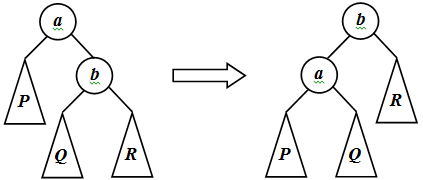
\includegraphics[width=0.5\linewidth]{small} \\ Малое правое вращение}
		\end{minipage}
		\hfill
		\begin{minipage}[h]{0.49\linewidth}
			\centering
			{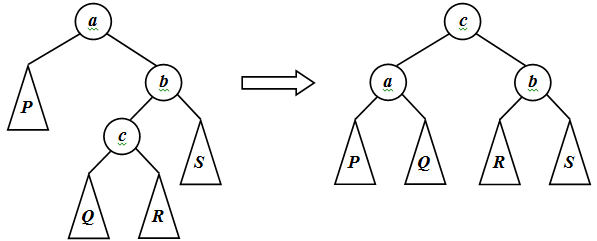
\includegraphics[width=0.5\linewidth]{big} \\ Большое правое вращение}
		\end{minipage}
		\caption{Иллюстрация вращений}
		\label{ris:image1}
	\end{figure}
	
	
	
\end{document}
